\chapter{基于蒙特卡洛采样的显著性区域检测}

\section{引言}
在上一章我们介绍了基于条件随机场的显著区域检测算法,虽然具有很高的准确率和召回率,但是其训练过程复杂耗时,在线检测的时间复杂度也较高。本章将介绍基于蒙特卡洛采样的显著区域检测方法,该方法在保持一定检测性能的同时,具有时间复杂度低,且易于并行化的优点,非常适合于实际工程。本节首先介绍了相关研究工作,然后探索了显著区域在空间上的几个特性(包络性、连通性,紧致性),并设计了基于蒙特卡洛采样的融合模型,有机地将这几种空间特性结合起来,生成最后的显著图。在本章的最后,我们在两个国际公开数据集上进行了实验,对比了十余种国际主流的显著区域检测算法。实验结果显示,我们的算法在保持足够检测性能的同时,拥有较低的时间复杂度和较高的并行计算能力。

\subsection{相关工作}
对视觉显著性的研究最早可以追溯到Koch和Ullman的基于生物视觉原理的模型\cite{koch1987shifts},之后Itti等人融入了多尺度图像特征进行了改进\cite{itti1998model}。自此之后,显著性检测就吸引了来自各个领域的众多学者。

在最初的阶段,人们试图根据局部对比度挖掘图像区块的稀有性,从而去定义显著值。在Ma和Zhang的工作中\cite{ma2003contrast},首次结合了fuzzy growing与局部对比度分析用于显著区域检测。在Harel等人的工作中\cite{harel2006graph},根据相邻像素点的相似性首先构建了一个邻接图,然后利用马尔科夫过程来挖掘像素的显著性。其他学者,比如Liu等人\cite{liu2011learning},以及Mai等人\cite{maisaliency},都将局部对比度作为一个很重要的特征。

然而,基于局部对比度的方法倾向于给予边缘更高的显著值,而并非高亮整个显著区域。故近年来,越来越多的学者开始使用全局对比度作为显著区域检测的重要特征。Zhai等人\cite{zhai2006visual}提出了第一个基于全局对比度的显著区域检测模型,然而,考虑到直接在三通道色彩空间上计算,时间复杂度太高,他们只采用了亮度信息进行计算。Cheng等人\cite{cheng2011global}则改进了这个算法,他们应用了三通道进行计算,为了减少时间复杂度,同时引入了颜色向量量化和色彩空间平滑两个工具。

随着机器学习方法的火热,机器学习也被许多学者尝试应用于该领域。Kienzel等人\cite{zhai2006visual}基于眼动数据学习了一个kernel SVM,用于区分一个图像块是否显著。Ye等人\cite{ye2014salient}则采用了条件随机场,将局部和全局特征相结合,以弥补各个特征的缺陷。

\subsection{显著性区域的空间约束特征}
当前国际上的主流方法均有各自的不足:基于局部对比度的方法倾向于高亮边缘,而基于全局对比度的方法无法区分前景和背景中相同颜色的像素,基于学习的方法严重依赖训练数据,在不同数据集上表现差异较大。

\begin{figure}
\centering
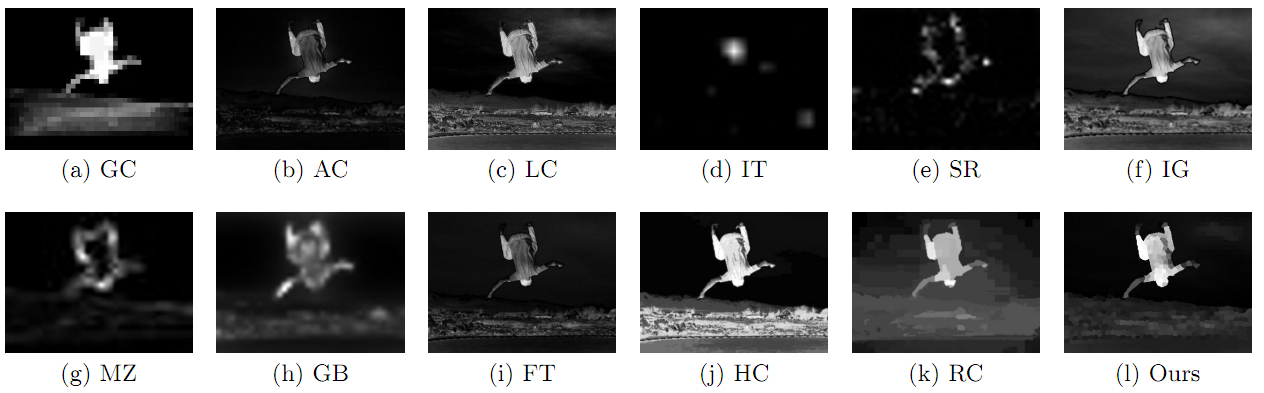
\includegraphics[width=\textwidth]{mcs-example.jpg}
\caption{与其余10种方法的对比示例}\label{fig:mcs_comp}
\end{figure}

我们通过对显著性区域的进一步观察与分析发现,显著区域存在一定的空间约束,利用这些空间约束特征,可以大大的提高显著区域检测的性能。如图\ref{fig:mcs_comp}所示,基于局部对比度的方法,如MZ\cite{ma2003contrast},倾向于高亮物体的边缘,而基于全局对比度的方法如HC\cite{cheng2011global},则会将草地也一起高亮(因为草地与前景颜色相近,相对于天空同样具有较大的对比度)。而实际上,这些方法都可以通过加入空间约束特征进行修正。首先,如果一个区域被显著的区域所包围,那么这个区域也通常是显著的,这可以解决基于局部对比度的方法的缺陷;其次,如果一个区域与图像的边框相连接,那么这个区域通常不是显著的,这可以一定程度上弥补基于全局对比度的方法的不足。

在我们的工作中,提出了三种空间约束关系:连通性、紧致性、包络性。然而,这三种空间特征都是二值特征,很难直接将其应用到显著图中。为此我们创造性的提出了蒙特卡洛采样的融合框架,将显著值的度量分解为多次采样-标记的过程。在接下来的部分,我们首先介绍了整个系统的框架结构,然后依次介绍采样方法和显著图的生成,同时,我们穿插引入了三种空间特征并将其应用到显著图的生成中。最后,我们通过实验验证了我们的方法的有效性。

\section{基于蒙特卡洛采样的显著区域检测}
\begin{figure}
\centering
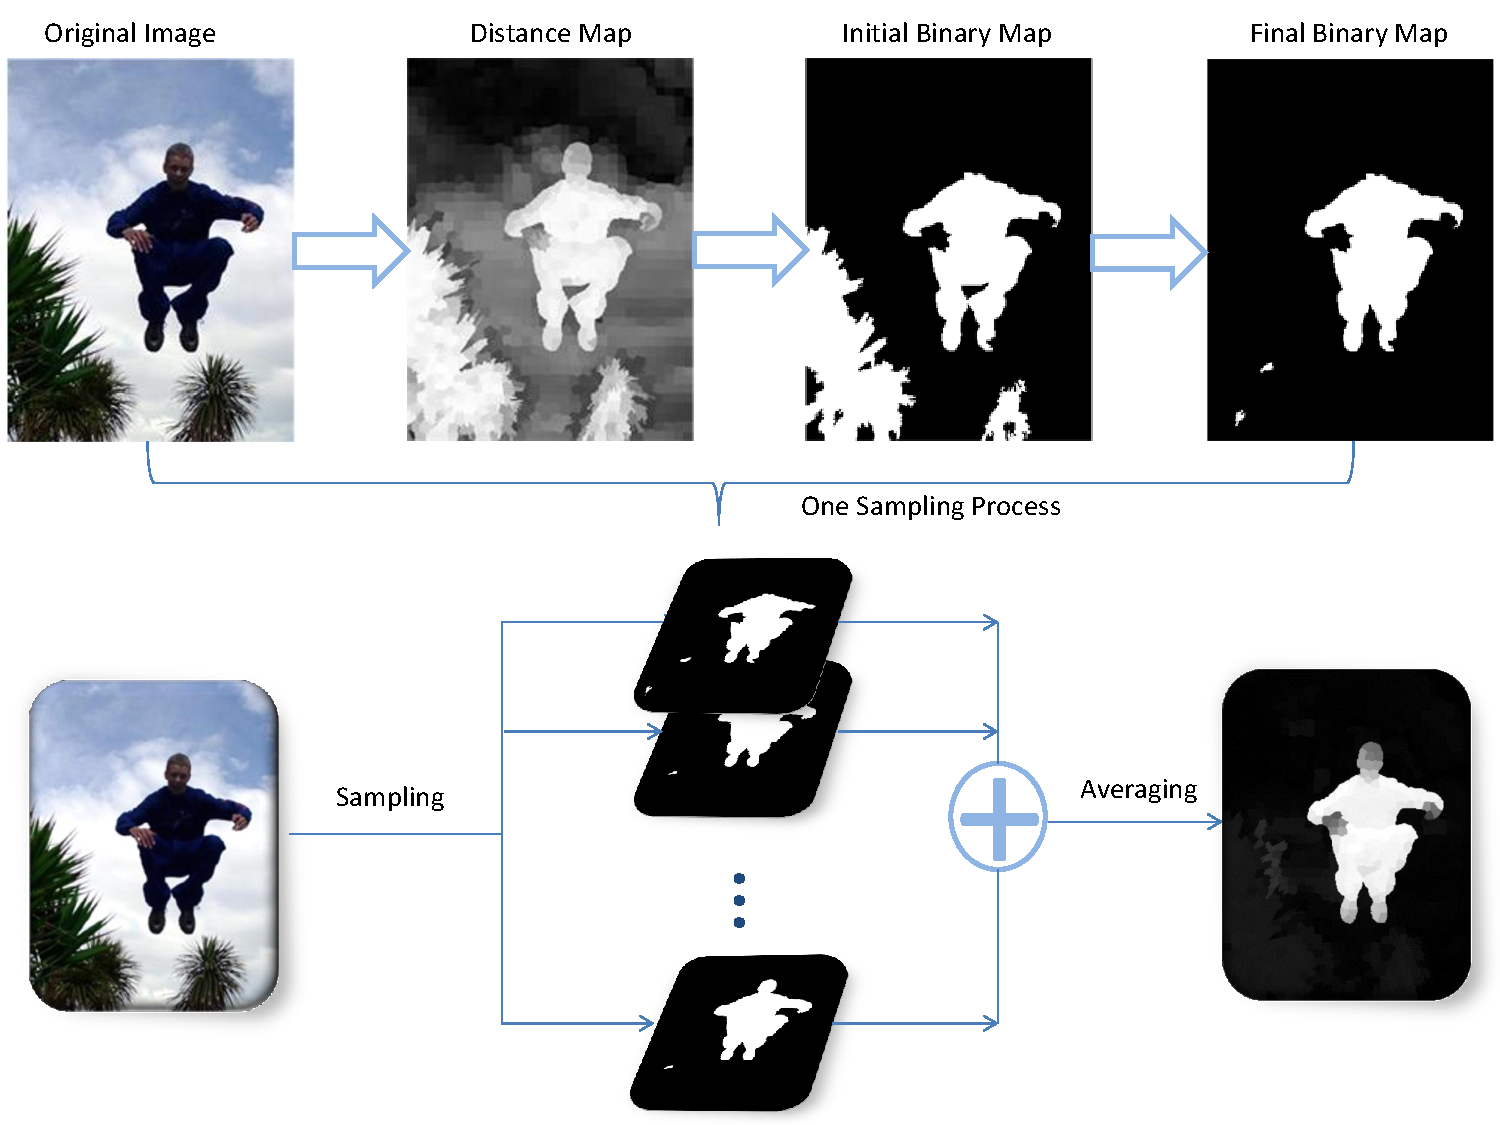
\includegraphics[width=\textwidth]{MCS.pdf}
\caption{系统框架图}\label{fig:mcs}
\end{figure}

我们的系统框架如图\ref{fig:mcs}所示。为了将三种空间特征利用起来,我们使用了蒙特卡洛采样,将显著值的度量分解为多次采样-标记的过程,主要步骤如下:
\begin{enumerate}
\item 采样。对整幅图像中的像素点,以一定概率分布进行采样,最终采样得到一个像素的颜色向量,留作后续处理。
\item 对采样进行处理。对采样得到的像素点,计算整幅图像的距离图,继而利用紧致性和连通性对距离图进行二值化,计算得到初始二值图,最后利用包络性计算最终的二值图。
\item 对多次采样得到的二值图进行加权平均,得到最终的显著图。
\end{enumerate}

接下来,我们将按照上述主要步骤,依次详细的介绍我们的显著区域检测方法。

\subsection{采样方法}
显著性区域检测和图像分割实际上非常相似,区别在于,前者仅仅将图像分割为两个部分:前景和背景。因此,在显著性区域检测中,图像的像素被自然的划分为前景和背景两类,显然,属于不同类别的像素点应该具有较大的差异,而属于同一类的像素点差异较小。根据我们的假设,为了高亮前景物体,我们应该在采样的时候尽量采样背景像素,这样得到的distance map中,前景物体则会被高亮,背景物体则会呈现灰暗。

根据心理学家的分析\cite{tatler2007central},人类的注意力倾向于图像中心区域,同时摄影师在摄影时,也倾向于将主体部分放置在靠近中心的位置。因此,靠近图像中心的像素点,有较大概率为前景像素点,而靠近图像边缘的像素点,则有较大概率为背景像素。因此,为了以较大概率采样得到背景像素点,我们将采样的概率分布设定如下:
\begin{equation}
p(I_i) = \frac{1}{Z}(1-exp\{-\lambda(x_i-x_c)^2\})
\end{equation}

这里,$I_i$代表图像中的第$i$个像素点,$p(I_i)$表示该像素点被采样到的概率,$x_i$是该点的坐标,$x_c$是图像中心的坐标,$Z$是归一化因子。

\subsection{距离图}
一旦我们采样得到一个像素点,我们就可以通过以下公式计算整幅图中其他像素点与这个像素的差异:
\begin{equation}
D(I_i) = ||f_i - f_s|| \label{eq:dis}
\end{equation}

这里$f_i$是第$i$个像素点的特征向量,$f_s$是采样点的特征向量。$||*||$为欧氏距离算子。在我们的工作中,我们选取Lab颜色空间的颜色向量作为特征向量。然后我们通过归一化,将其归一化到0和1之间,得到距离图。

由于在得到的距离图中,存在一些异常高的值,因而使用通常的MIN-MAX归一化会使某些单一的像素高亮,而整幅图像比较暗淡。因此,我们采用下面的方法进行归一化:
\begin{equation}
D = 
\begin{cases}
1& d \geq a\\
(d-u)/(a-u) & u<d<a\\
0& d \leq u
\end{cases}
\end{equation}

这里$d$是由公式\ref{eq:dis}计算得到的距离,$a$和$u$都是根据图像内容自适应的像素值参数。$a$被设置为使至少有5\%的像素值大于$a$,$u$被设置为至少有5\%的像素值小于$u$。

\subsection{初始二值标记图}
我们通过阈值化distance map获得二值标记图,如下所示:
\begin{equation}
B(I)= \textbf{THRESH}(D(I), \theta)
\end{equation}

然而,如何选取一个合适的阈值是非常困难的事情。如前文所述,我们的方法结合了三种空间特征,在这里,我们使用紧致性和连通性来确定一个合适的阈值,得到初始二值标记图后,我们再利用包络性优化该图,得到最终的二值标记图。

根据我们的观察,一个二值图标记的显著区域通常比较集中,且形成一个连通的区域。我们将二值图在空间上分布的方差作为考量紧致性的指标:
\begin{equation}
BinMap_{Var} = Var_X + Var_Y
\end{equation}
其中
\begin{equation}
Var_X = \frac{1}{N} \sum_{i=1}^N |x_i-x_c|
\end{equation}
\begin{equation}
Var_Y = \frac{1}{N} \sum_{i=1}^N |y_i-y_c|
\end{equation}

$N$是被标记为显著的像素数量,$(x_i,y_i)$则是第$i$个像素的坐标,$(x_c,y_c)$是所有被标记为显著的像素的中心。

对于连通性,我们考虑显著像素的8邻域内显著像素的数量,数量越多,说明连通性越好:
\begin{equation}
BinMap_{Con} = \frac{1}{N}\sum_{p\in I_{Sal}}\sum_{(x,y)\in N_p}\emph{1}(p_{xy})
\end{equation}

其中,$I_{Sal}$为二值图中显著像素的集合,N是该集合的大小,$N_p$是像素$p$的8邻域的坐标,$1(p_{xy})$则是判定函数,用于判定在$(x,y)$的像素点$p_{xy}$是否为显著像素。

显然,高连通性,空间分布越集中的二值图更能有效的标记一个显著性区域,因此,我们的阈值通过以下公式确定:
\begin{equation}
Criterion = \frac{BinMap_{Con}}{BinMap_{Var}}
\end{equation}
在我们的实现中,我们均匀选取了9个不同的阈值,并获得了9幅不同的显著图,然后,我们通过上面的式子,将$Criterion$最高的显著图选取为初始的二值标记图。

\subsection{二值标记图}
通过包络性,我们可以进一步优化二值标记图。根据Gestalt原理\cite{beardslee1958readings},一个有着封闭轮廓的区域更加易于被人眼理解为一个整体的实物,因而吸引人眼的注意力。

\begin{figure}
\centering
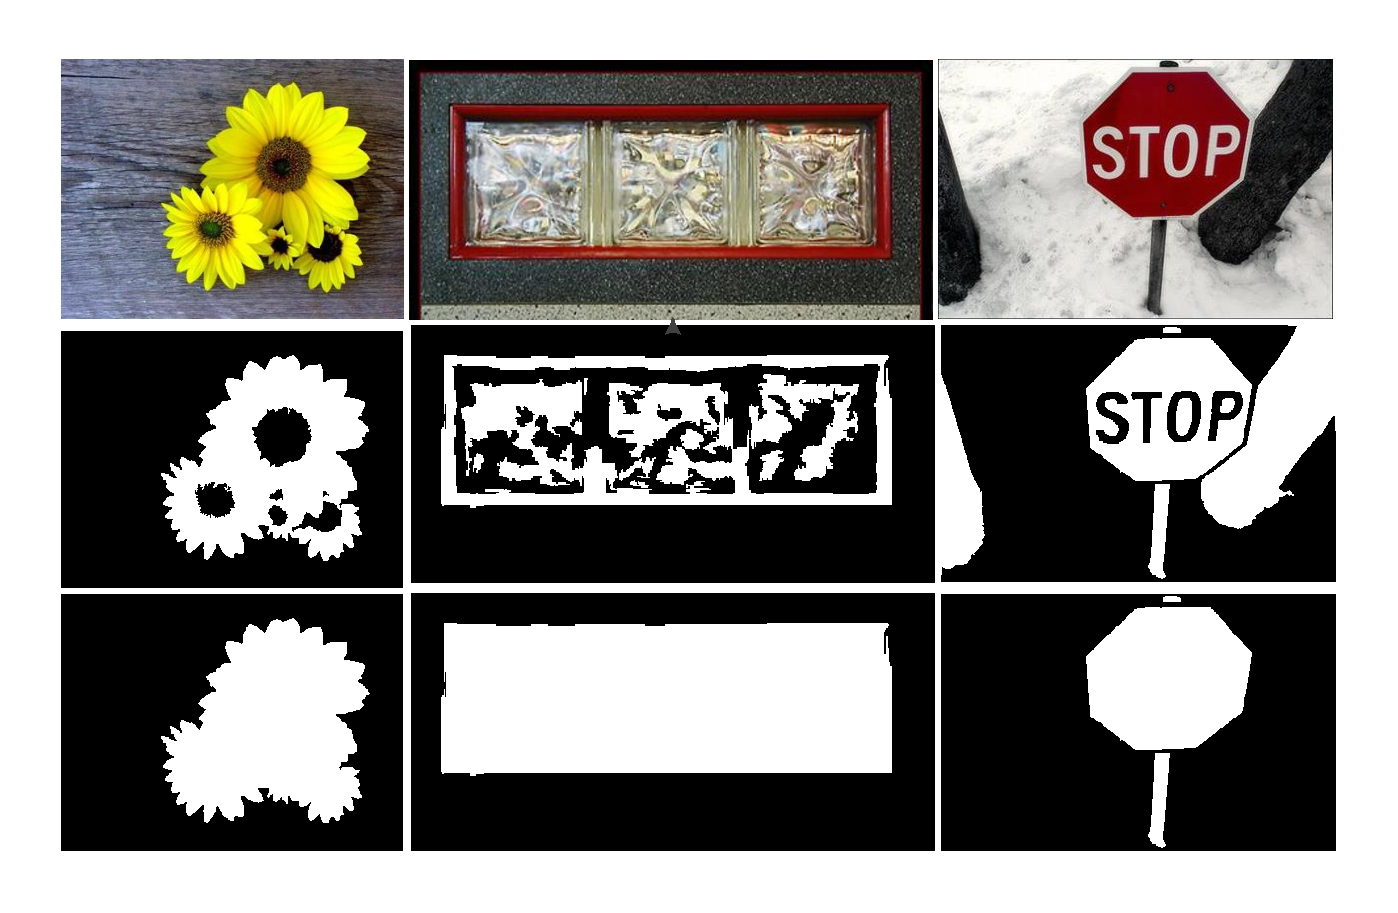
\includegraphics[width=\textwidth]{constraint.pdf}
\caption{包络性的作用} \label{fig:constraint}
\end{figure}

我们将包络性定义为二值图中有着封闭轮廓的区域,在这个定义下,任何与图像边缘连通的区域将被标记为0(背景区域),其余的区域则被标记为1(前景区域)。我们可以通过泛洪法填充,在$O(n)$的时间内标记出所有的像素点。

在图\ref{fig:constraint}中,上面一行为原图像,中间一行为初始二值标记图,下面一行为通过包络性优化过的最终的二值标记图,可以看到,通过这一简单的优化,可以大大提高二值标记图的质量。

\subsection{显著图}
在每一次采样后,我们都会得到一幅二值标记图,其中1标记为这次采样中,认为该像素为显著区域,0标记为在这次采样中,认为该像素为非显著区域。根据蒙特卡洛采样原理,一个像素的显著值(即它被标记为显著的概率)最终可以用整个采样过程中,其被标记为1的频率替代(当采样次数足够多时)。因此,我们最后简单的将所有得到的二值图进行加和平均,即:
\begin{equation}
Sal(I) = \frac{1}{T}\sum_{i=1}^{N}BinMap_i(I)
\end{equation}

其中$Sal(I)$即图像$I$的显著图,$T$是采样的次数,$BinMap_i(I)$是在第$i$次采样过程中得到的二值图。在我们的实现中,我们设置$T=400$。

\section{实验及分析}
我们分别在ASD\cite{achanta2009frequency}和ECSSD\cite{yan2013hierarchical}这两个公开数据集上进行了我们的实验。同时与11中国际经典算法进行了对比,包括IT98\cite{itti1998model}, MZ03\cite{ma2003contrast}, LC06\cite{zhai2006visual}, GB06\cite{harel2006graph}, SR07\cite{hou2007saliency},  AC08\cite{achanta2008salient}, FT09\cite{achanta2009frequency},  IG09\cite{achanta2009frequency}, HC11\cite{cheng2011global}, RC11\cite{cheng2011global}, and GS12\cite{wei2012geodesic}。在接下来的部分,我们分别展示了在ASD和ECSSD两个数据集上的实验结果并进行了分析,在本节的最后还对我们的算法效率进行了分析优化。

\subsection{在ASD数据集上的结果}
\begin{figure}
\centering
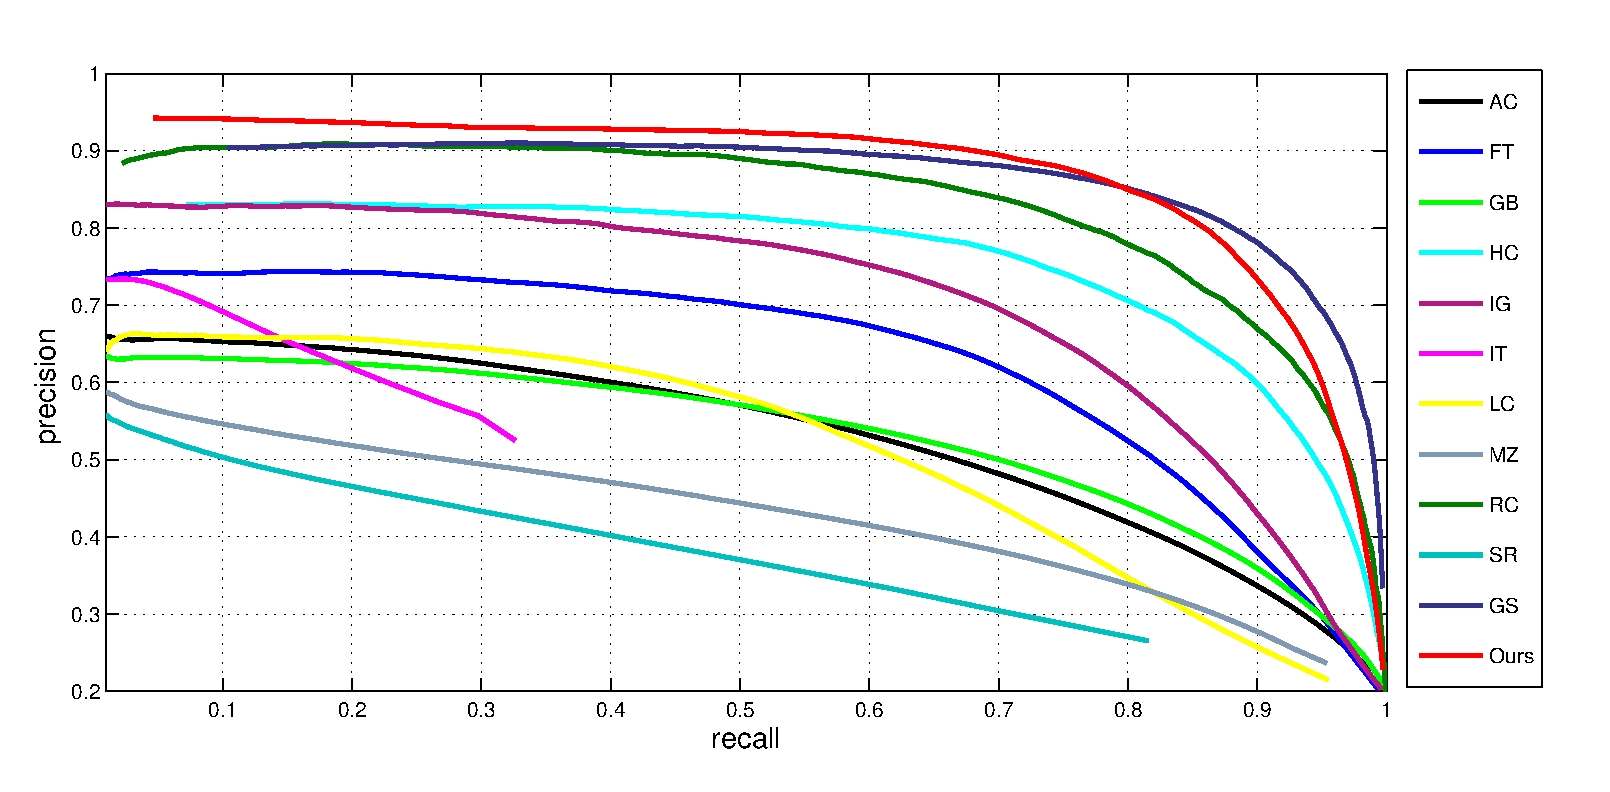
\includegraphics[width=\textwidth]{mcs_pr_curve.eps}
\caption{ASD数据集上与其他10种方法的对比:准确率-召回率曲线}
\label{fig:results2_pr}
\end{figure}
\begin{figure}
\centering
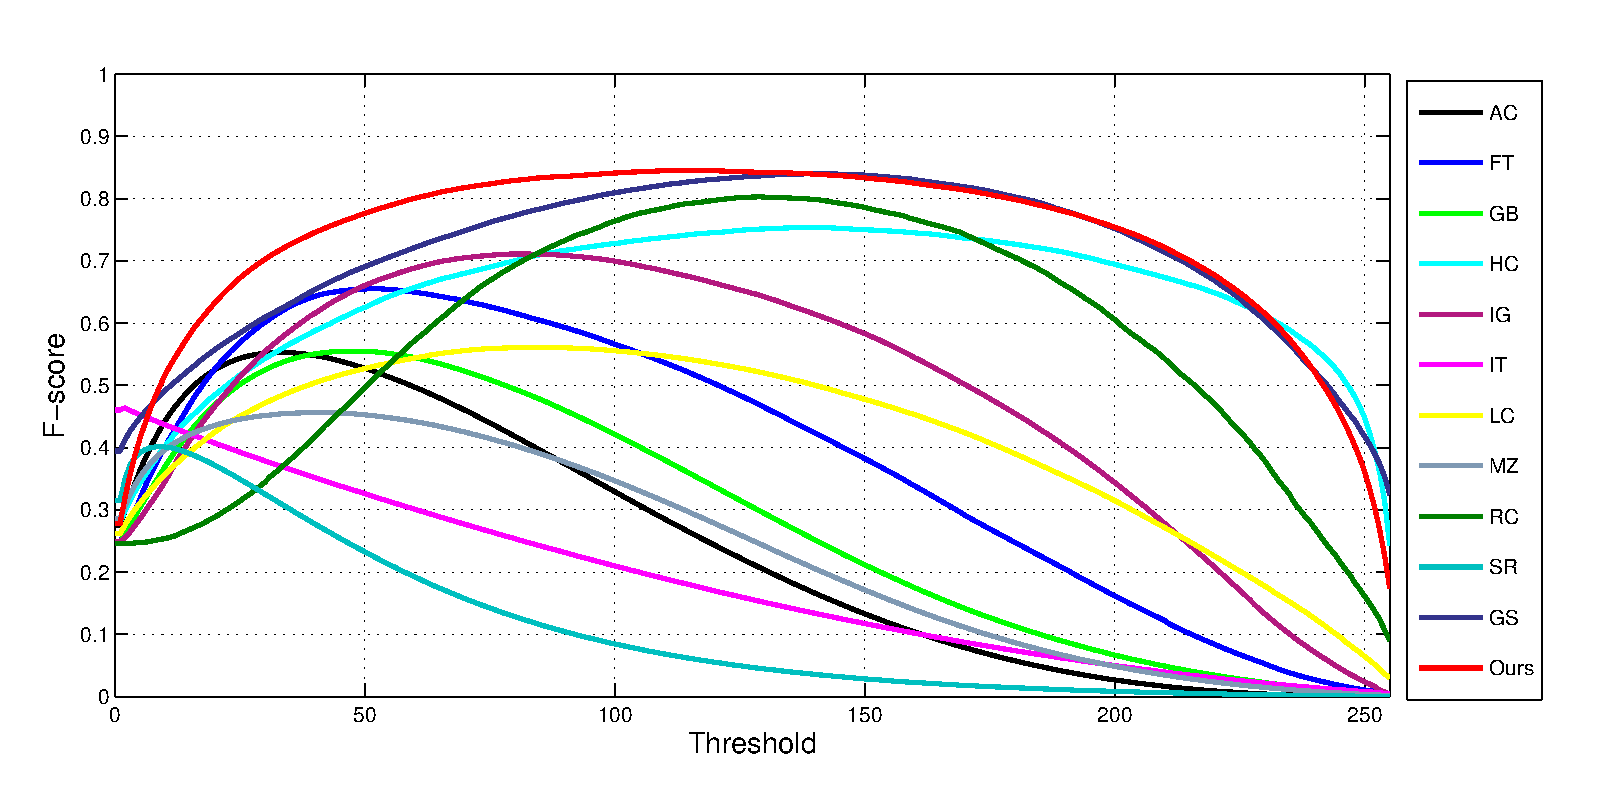
\includegraphics[width=\textwidth]{mcs_f.eps}
\caption{ASD数据集上与其他10种方法的对比:F-score曲线}
\label{fig:results2_fscore}
\end{figure}
\begin{figure}
\centering
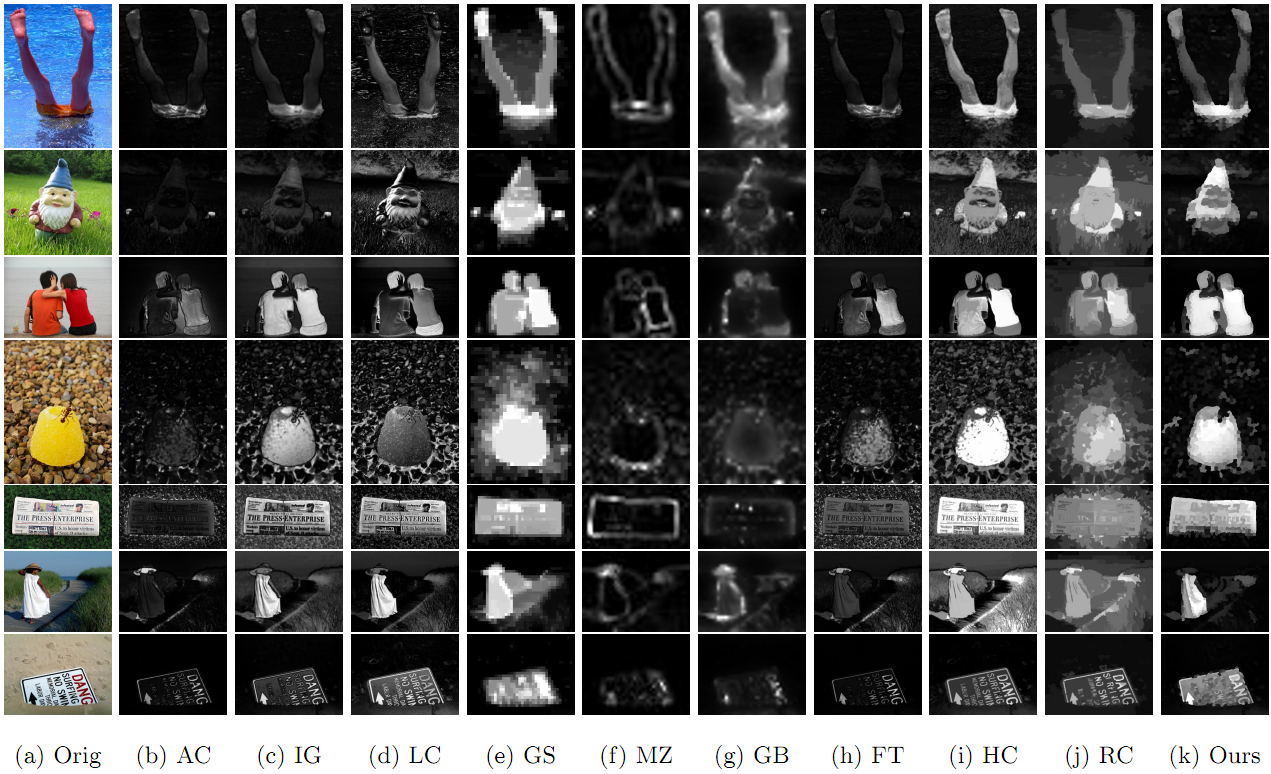
\includegraphics[width=\textwidth]{mcs_vcomp.jpg}
\caption{ASD数据集上与其他10种方法的主观视觉对比}\label{fig:vresult2}
\end{figure}

可以看到,我们的方法在ASD数据集上有着良好的表现,与GS方法有非常接近的性能。尽管GS方法在召回率大于0.8的时候有更高的准确率,我们的方法在召回率低于0.8时,拥有更高的性能。同时,从F-score中可以看到,我们的方法在很大的阈值范围内均有非常良好的表现,这说明了我们的方法对阈值的选取不敏感,具有较高的鲁棒性。

\subsection{在ECSSD数据集上的结果}
\begin{figure}
\centering
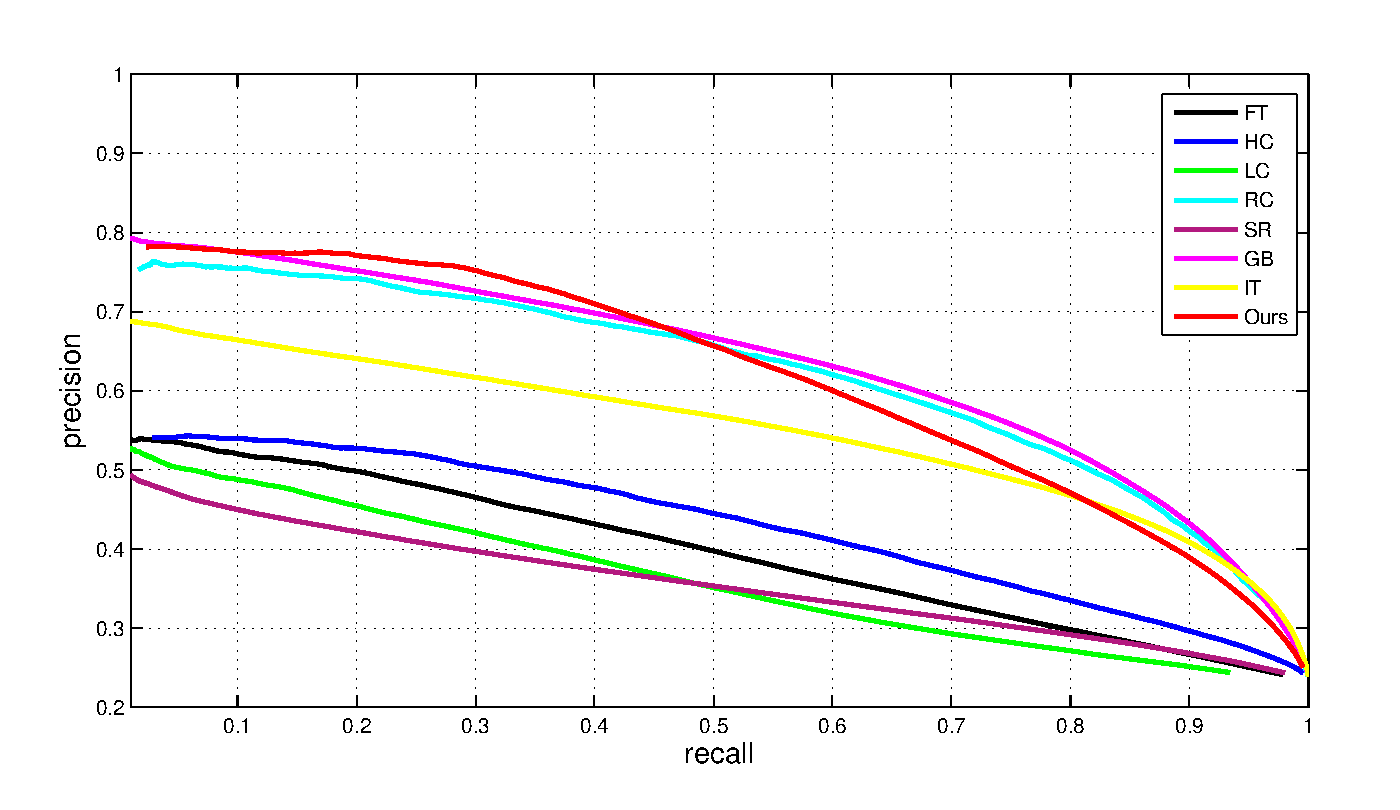
\includegraphics[width=\textwidth]{pr_curve_ecssd.eps}
\caption{ECSSD数据集上与其他10种方法的对比:准确率-召回率曲线}
\label{fig:results2_pr_ecssd}
\end{figure}
\begin{figure}
\centering
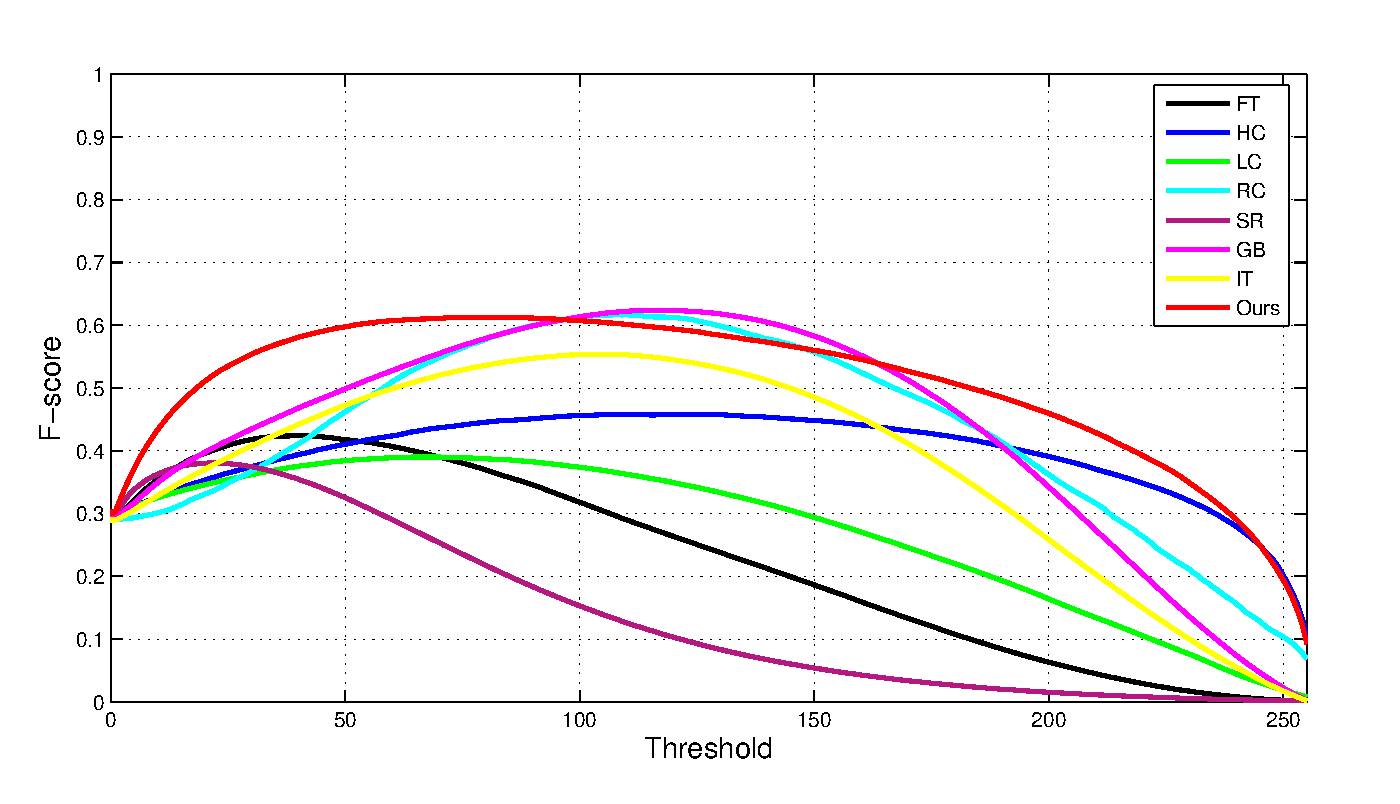
\includegraphics[width=\textwidth]{f_ecssd.eps}
\caption{ECSSD数据集上与其他10种方法的对比:F-score曲线}
\label{fig:results2_fscore_ecssd}
\end{figure}
\begin{figure}
\centering
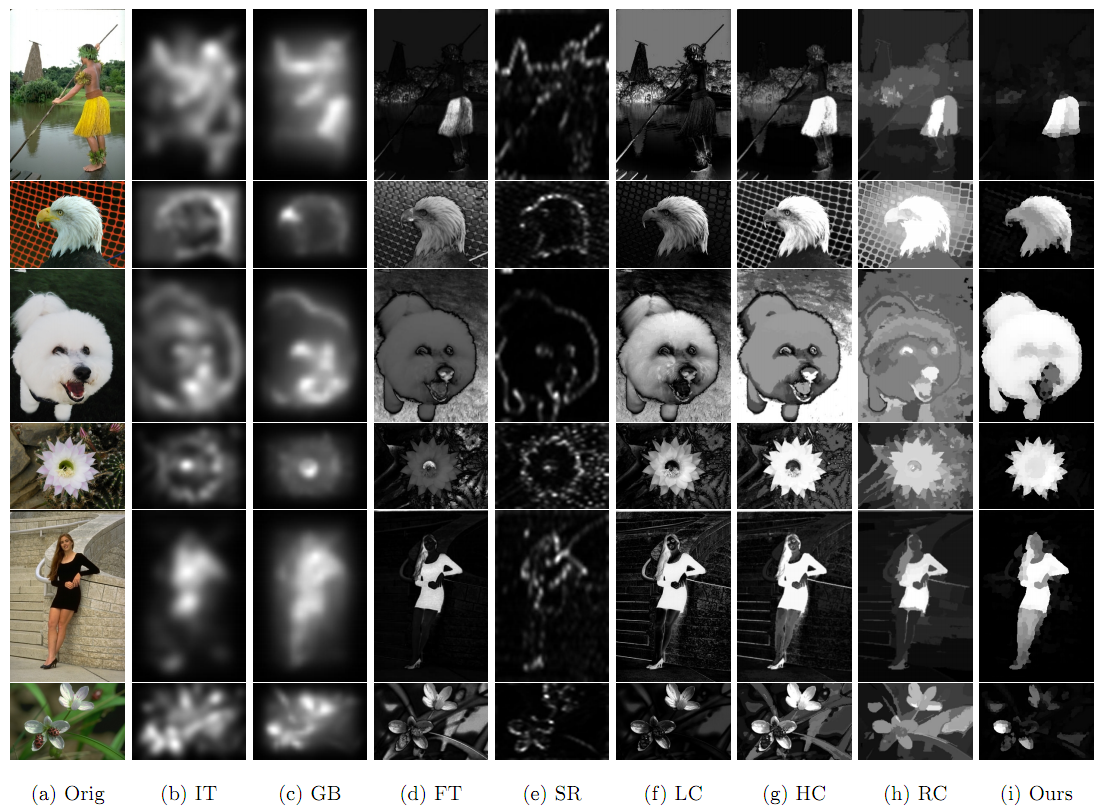
\includegraphics[width=\textwidth]{vresult_ecssd.png}
\caption{ECSSD数据集上与其他10种方法的主观视觉对比}\label{fig:vresult2_ecssd}
\end{figure}

ECSSD是一个更加有挑战性的数据集,包含了1000幅背景结构复杂的图片。由于找不到AC,IG,GS方法在这个数据集上的结果,作者也没有公开源码,因此我们仅仅比较剩余的方法。

从图\ref{fig:results2_pr_ecssd}和图\ref{fig:results2_fscore_ecssd}可以看到,我们的方法在这个数据集上依然保持竞争力。显然,由于数据集的背景结构更加复杂,所有的方法在这个数据集上的表现都有所下降。在图\ref{fig:vresult2_ecssd}中,我们列出了两个我们的方法表现较差的图像(第一行和最后一行)。在这样的图像中,前景图像要么对比度很低(比如第一行中人的身体),要么空间先验不起作用(比如最后一行中,花朵与图像的边缘连接在了一起)。在这类图像中,包括对比度、纹理等在内的底层视觉特征已经不能有效的体现人眼视觉特性,导致在显著区域的识别上准确率严重降低。

\subsection{算法优化}
对于我们的算法,如果直接在原图像上去进行上面的计算,由于像素数量很多,会导致时间复杂度极高。为了加速上述采样过程,我们使用了以下两个算法进行加速:
\begin{enumerate}
\item SLIC超像素分割算法\cite{achanta2010slic}。我们将整幅图像分割为超像素,之后所有的计算都以超像素为基本单元进行计算,这样可以使得像素数量显著下降。典型地,一幅400x300分辨率的图像,经过超像素分割后,最终形成大约400个左右的超像素单元。
\item 并行采样。由于每一次采样过程都是相互独立的,因此可以非常方便的将所有采样过程并行计算。由于我们的测试环境为4核cpu,我们将采样的线程数设置为4。
\end{enumerate}

进行效率优化后,我们的算法具有很高的计算效率,时间复杂度大大降低。我们在表\ref{tab:eff}中对比了HC, RC和我们的方法(ST表示我们的单线程版本,FT表示我们的四线程版本),从表中可以看到,我们的方法在多线程时具有很高的时间效率,与表现相当的RC方法相比,我们的时间消耗减少了60\%以上。

\begin{table}
\centering
\vspace{0.06in}
\begin{tabular}{|c|c|c|c|c|}\hline
Method & HC   & RC   & Ours(ST) & Ours(FT)\\\hline
Time(s)& 0.013& 0.192& 0.207    & 0.061   \\\hline
\end{tabular}
\caption{时间效率比较}\label{tab:eff}
\end{table}